\subtitle{\bf Aula 9 - Motiva\c{c}
\begin{frame}[t,plain]
\titlepage
\end{frame}

\begin{frame}{Objetivos}
\protect\hypertarget{objetivos-1}{}
\begin{itemize}
\item
  Apresentar a estratégia de análise bottom-up
\item
  Apresentar 3 algoritmos: Earley, LR(0) e SLR.
\end{itemize}
\end{frame}

\hypertarget{motivauxe7uxe3o}{%
\section{Motiva\c{c}\~{a}o}\label{motivauxe7uxe3o}}

\begin{frame}{Limita\c{c}\~{o}es: Top-Down}
\protect\hypertarget{limitauxe7uxf5es-top-down}{}
\begin{itemize}

\item
  Analisadores \textbf{LL} exigem transforma\c{c}\~{o}es na gramática

  \begin{itemize}

  \item
    Remo\c{c}\~{a}o de recurs\~{a}o \`{a} esquerda
  \item
    Fatora\c{c}\~{a}o \`{a} esquerda
  \end{itemize}
\end{itemize}
\end{frame}

\begin{frame}{Limita\c{c}\~{o}es: Top-Down}
\protect\hypertarget{limitauxe7uxf5es-top-down-1}{}
\begin{itemize}

\item
  Decis\~{a}o com apenas \textbf{1 token de lookahead}
\item
  Algumas gramáticas s\~{a}o inerentemente n\~{a}o-LL(1)
\end{itemize}
\end{frame}

\begin{frame}{A Ideia Bottom-Up}
\protect\hypertarget{a-ideia-bottom-up}{}
\begin{itemize}

\item
  Analisadores \textbf{bottom-up} l\^{e}em um prefixo maior antes de decidir
\item
  Suportam \textbf{recurs\~{a}o \`{a} esquerda} naturalmente
\end{itemize}
\end{frame}

\begin{frame}{A Ideia Bottom-Up}
\protect\hypertarget{a-ideia-bottom-up-1}{}
\begin{itemize}

\item
  Constroem uma \textbf{deriva\c{c}\~{a}o mais \`{a} direita invertida}
\item
  Cada redu\c{c}\~{a}o constrói um peda\c{c}o da árvore sintática
\end{itemize}
\end{frame}

\begin{frame}{Der. \`{a} Direita Invert.}
\protect\hypertarget{der.-uxe0-direita-invert.}{}
Gramática de exemplo (n\~{a}o-LL(1)):

\[\begin{array}{lcl}
S &\to& S + E \mid E \\
E &\to& (S) \mid n
\end{array}\]
\end{frame}

\begin{frame}[fragile]{Der. \`{a} Direita Invert.}
\protect\hypertarget{der.-uxe0-direita-invert.-1}{}
Analisando \texttt{(1) + 2}:

\begin{lstlisting}
S'  =>  S  =>  S+E  =>  S+2  =>  E+2  →  (S)+2  =>  (E)+2  =>  (1)+2
\end{lstlisting}

O analisador constrói essa deriva\c{c}\~{a}o de baixo para cima, da direita para
a esquerda.
\end{frame}



\begin{frame}{A Ideia Central}
\protect\hypertarget{a-ideia-central}{}
\begin{itemize}

\item
  Simula \textbf{todas as análises possíveis} em paralelo
\item
  Em vez de se comprometer com uma produ\c{c}\~{a}o, prev\^{e} todas
\item
  Usa \textbf{compartilhamento de trabalho} para efici\^{e}ncia polinomial
\item
  Processa cada posi\c{c}\~{a}o de entrada \(j\) mantendo um conjunto \(I_j\) de
  \textbf{itens}
\end{itemize}
\end{frame}

\begin{frame}{Itens Earley}
\protect\hypertarget{itens-earley}{}
Um item Earley \([A \to \beta . \gamma, k]\) representa:

\begin{itemize}

\item
  \(A \to \beta\gamma\): produ\c{c}\~{a}o sendo usada
\item
  \(.\) (ponto): posi\c{c}\~{a}o atual no reconhecimento
\item
  \(k\): posi\c{c}\~{a}o na entrada onde o reconhecimento de \(A\) come\c{c}ou
\end{itemize}
\end{frame}

\begin{frame}[fragile]{Exemplos}
\protect\hypertarget{exemplos}{}
\begin{itemize}

\item
  \([E \to . (S), 0]\): come\c{c}amos a reconhecer \(E \to (S)\) na posi\c{c}\~{a}o
  0, nada visto ainda
\item
  \([E \to ( S . ), 0]\): vimos \texttt{(S}, esperamos
  \texttt{)}
\item
  \([E \to (S) ., 0]\): \(E\) completamente reconhecida a partir da
  posi\c{c}\~{a}o 0
\end{itemize}
\end{frame}

\begin{frame}{Algoritmo de Earley}
\protect\hypertarget{algoritmo-de-earley-1}{}
\textbf{Inicializa\c{c}\~{a}o:} \(I_0 = \{[S' \to . S, 0]\}\)
\end{frame}

\begin{frame}{Algoritmo de Earley}
\protect\hypertarget{algoritmo-de-earley-2}{}
\begin{enumerate}

\item
  \textbf{Predi\c{c}\~{a}o}: se \([A \to \alpha . B \beta, k] \in I_j\) e
  \(B \to \gamma\) é uma produ\c{c}\~{a}o, adiciona \([B \to . \gamma, j]\) a
  \(I_j\)
\end{enumerate}
\end{frame}

\begin{frame}{Algoritmo de Earley}
\protect\hypertarget{algoritmo-de-earley-3}{}
\begin{enumerate}
\setcounter{enumi}{1}

\item
  \textbf{Verificar (scan)}: se \([A \to \alpha . a \beta, k] \in I_j\)
  e o token atual é \(a\), adiciona \([A \to \alpha\, a . \beta, k]\) a
  \(I_{j+1}\)
\end{enumerate}
\end{frame}

\begin{frame}{Algoritmo de Earley}
\protect\hypertarget{algoritmo-de-earley-4}{}
\begin{enumerate}
\setcounter{enumi}{2}

\item
  \textbf{Completar}: se \([B \to \gamma ., k] \in I_j\), para cada
  \([A \to \alpha . B \beta, l] \in I_k\), adiciona
  \([A \to \alpha\, B . \beta, l]\) a \(I_j\)
\end{enumerate}
\end{frame}

\begin{frame}{Algoritmo de Earley}
\protect\hypertarget{algoritmo-de-earley-5}{}
\textbf{Aceita:} se \([S' \to S ., 0] \in I_n\)
\end{frame}

\begin{frame}{Exemplo: Análise de \texttt{(1) + 2}}
\protect\hypertarget{exemplo-anuxe1lise-de-1-2}{}
Gramática: \(S \to S+E \mid E\) e \(E \to (S) \mid n\)

\begin{table}
\begin{tabular}[]{@{}llll@{}}
\toprule
Conjunto & Item & Pos & Motivo \\
\midrule

\(I_0\) & \(S' \to . S\) & 0 & inicial \\
& \(S \to . S+E\) & 0 & prever \(S\) \\
& \(S \to . E\) & 0 & prever \(S\) \\
& \(E \to . n\) & 0 & prever \(E\) \\
& \(E \to . (S)\) & 0 & prever \(E\) \\
\bottomrule
\end{tabular}
\end{table}
\end{frame}

\begin{frame}[fragile]{Exemplo: Análise de
\texttt{(1) + 2}}
\protect\hypertarget{exemplo-anuxe1lise-de-1-2-1}{}
Gramática: \(S \to S+E \mid E\) e \(E \to (S) \mid n\)

\begin{table}
\begin{tabular}[]{@{}llll@{}}
\toprule
Conjunto & Item & Pos & Motivo \\
\midrule

\(I_1\) & \(E \to ( . S )\) & 0 & consumir
\texttt{(} \\
& \(S \to . S+E\) & 1 & prever \(S\) \\
& \(S \to . E\) & 1 & prever \(S\) \\
& \(E \to . n\) & 1 & prever \(E\) \\
& \(E \to . (S)\) & 1 & prever \(E\) \\
\bottomrule
\end{tabular}
\end{table}
\end{frame}

\begin{frame}[fragile]{Exemplo: Análise de
\texttt{(1) + 2} (continua\c{c}\~{a}o)}
\protect\hypertarget{exemplo-anuxe1lise-de-1-2-continuauxe7uxe3o}{}
\begin{table}
\begin{tabular}[]{@{}llll@{}}
\toprule
Conjunto & Item & Pos & Motivo \\
\midrule

\(I_2\) & \(E \to n .\) & 1 & consumir \texttt{1} \\
& \(S \to E .\) & 1 & completar \(E\) \\
& \(E \to (S . )\) & 0 & completar \(S\) \\
& \(S \to S . +E\) & 1 & completar \(S\) \\
\bottomrule
\end{tabular}
\end{table}
\end{frame}

\begin{frame}[fragile]{Exemplo: Análise de
\texttt{(1) + 2} (continua\c{c}\~{a}o)}
\protect\hypertarget{exemplo-anuxe1lise-de-1-2-continuauxe7uxe3o-1}{}
\begin{table}
\begin{tabular}[]{@{}llll@{}}
\toprule
Conjunto & Item & Pos & Motivo \\
\midrule

\(I_3\) & \(E \to (S) .\) & 0 & consumir \texttt{)} \\
& \(S \to E .\) & 0 & completar \(E\) \\
& \(S' \to S .\) & 0 & completar \(S\) \\
& \(S \to S . +E\) & 0 & completar \(S\) \\
\bottomrule
\end{tabular}
\end{table}
\end{frame}

\begin{frame}[fragile]{Exemplo: Análise de
\texttt{(1) + 2} (continua\c{c}\~{a}o)}
\protect\hypertarget{exemplo-anuxe1lise-de-1-2-continuauxe7uxe3o-2}{}
\begin{table}
\begin{tabular}[]{@{}llll@{}}
\toprule
Conjunto & Item & Pos & Motivo \\
\midrule

\(I_4\) & \(S \to S+ . E\) & 0 & consumir \texttt{+} \\
& \(E \to . n\) & 4 & prever \(E\) \\
\(I_5\) & \(E \to n .\) & 4 & consumir \texttt{2} \\
& \(S \to S+E .\) & 0 & completar \(E\) \\
& \(S' \to S .\) & 0 & completar \(S\): \textbf{sucesso!} \\
\bottomrule
\end{tabular}
\end{table}
\end{frame}

\begin{frame}{Visualiza\c{c}\~{a}o do Algoritmo de Earley}
\protect\hypertarget{visualizauxe7uxe3o-do-algoritmo-de-earley}{}
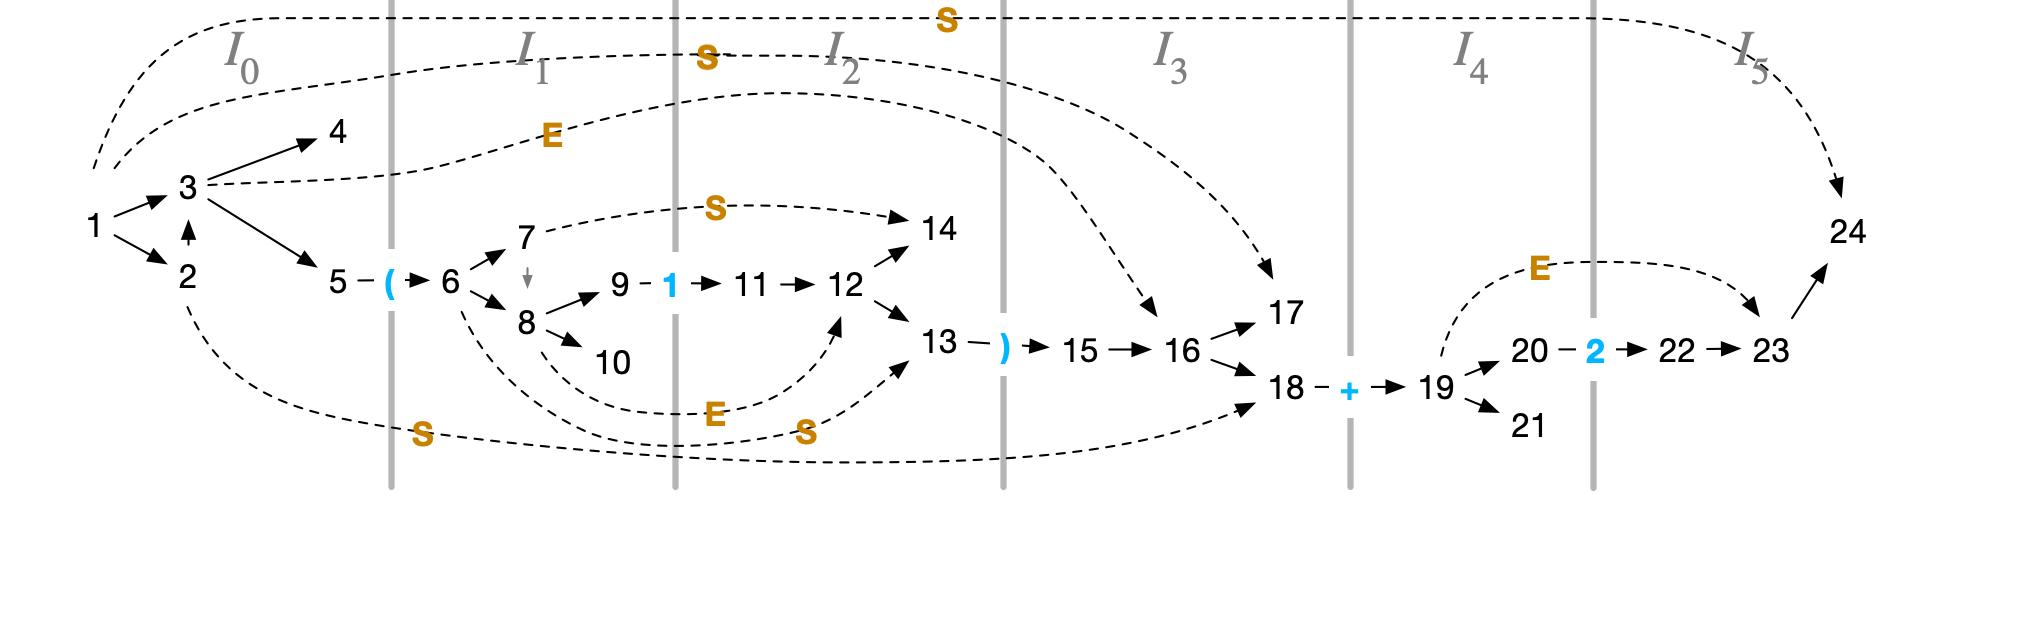
\includegraphics[width=\textwidth,height=0.82\textheight,keepaspectratio]{chapter09/imgs/earley-threads.png}
\end{frame}

\begin{frame}{Complexidade}
\protect\hypertarget{complexidade}{}
\begin{itemize}

\item
  \textbf{Pior caso geral}: \(O(n^3)\) --- inclui gramáticas ambíguas
\item
  \textbf{Gramáticas n\~{a}o-ambíguas}: \(O(n^2)\) no pior caso
\item
  \textbf{Gramáticas LL/LR}: \(O(n)\) quando implementado cuidadosamente
\end{itemize}
\end{frame}

\begin{frame}{Vantagens}
\protect\hypertarget{vantagens}{}
\begin{itemize}

\item
  Analisa \textbf{qualquer GLC}, incluindo ambíguas
\item
  Sem necessidade de transformar a gramática
\item
  Otimiza\c{c}\~{a}o de Aycock-Horspool: apenas 50\% mais lento que LALR
\end{itemize}
\end{frame}

\hypertarget{analisadores-lr-shift-reduce}{%
\section{Analisadores LR:
Shift-Reduce}\label{analisadores-lr-shift-reduce}}

\begin{frame}{A Ideia Shift-Reduce}
\protect\hypertarget{a-ideia-shift-reduce}{}
LR pode ser visto como uma \textbf{otimiza\c{c}\~{a}o do Earley}:

\begin{itemize}

\item
  As previs\~{o}es s\~{a}o \textbf{pré-computadas} como estados de um aut\^{o}mato
\end{itemize}
\end{frame}

\begin{frame}{A Ideia Shift-Reduce}
\protect\hypertarget{a-ideia-shift-reduce-1}{}
\begin{itemize}

\item
  Estado do analisador: uma \textbf{pilha de estados}
\item
  Duas a\c{c}\~{o}es: \textbf{shift} (consumir token) e \textbf{reduce} (aplicar
  produ\c{c}\~{a}o)
\end{itemize}
\end{frame}

\begin{frame}{A Ideia Shift-Reduce}
\protect\hypertarget{a-ideia-shift-reduce-2}{}
Em qualquer ponto:
\(\underbrace{\alpha}_{\text{pilha}} \cdot \underbrace{\beta}_{\text{entrada}}\)
é uma forma sentencial direita
\end{frame}

\begin{frame}[fragile]{Trace Shift-Reduce para
\texttt{(1)+2}}
\protect\hypertarget{trace-shift-reduce-para-12}{}
\begin{table}
\begin{tabular}[]{@{}lll@{}}
\toprule
Pilha & Entrada & A\c{c}\~{a}o \\
\midrule

& \texttt{(1)+2} & shift \\
\texttt{(} & \texttt{1)+2} & shift \\
\texttt{(1} & \texttt{)+2} & reduce
\(E \to n\) \\
\bottomrule
\end{tabular}
\end{table}
\end{frame}

\begin{frame}[fragile]{Trace Shift-Reduce para
\texttt{(1)+2}}
\protect\hypertarget{trace-shift-reduce-para-12-1}{}
\begin{table}
\begin{tabular}[]{@{}lll@{}}
\toprule
Pilha & Entrada & A\c{c}\~{a}o \\
\midrule

\texttt{(1} & \texttt{)+2} & reduce
\(E \to n\) \\
\texttt{(E} & \texttt{)+2} & reduce
\(S \to E\) \\
\texttt{(S} & \texttt{)+2} & shift \\
\bottomrule
\end{tabular}
\end{table}
\end{frame}

\begin{frame}[fragile]{Trace Shift-Reduce para
\texttt{(1)+2}}
\protect\hypertarget{trace-shift-reduce-para-12-2}{}
\begin{table}
\begin{tabular}[]{@{}lll@{}}
\toprule
Pilha & Entrada & A\c{c}\~{a}o \\
\midrule

\texttt{E} & \texttt{+2} & reduce
\(S \to E\) \\
\texttt{S} & \texttt{+2} & shift \\
\texttt{S+} & \texttt{2} & shift \\
\bottomrule
\end{tabular}
\end{table}
\end{frame}

\begin{frame}[fragile]{Trace Shift-Reduce para
\texttt{(1)+2}}
\protect\hypertarget{trace-shift-reduce-para-12-3}{}
\begin{table}
\begin{tabular}[]{@{}lll@{}}
\toprule
Pilha & Entrada & A\c{c}\~{a}o \\
\midrule

\texttt{S+2} & \texttt{$} & reduce
\(E \to n\) \\
\texttt{S+E} & \texttt{$} & reduce
\(S \to S+E\) \\
\texttt{S} & \texttt{$} &
\textbf{aceitar} \\
\bottomrule
\end{tabular}
\end{table}
\end{frame}

\begin{frame}{Decis\~{a}o: Quando Shift ou Reduce?}
\protect\hypertarget{decisuxe3o-quando-shift-ou-reduce}{}
\begin{itemize}

\item
  O analisador precisa decidir quando olha o topo da pilha e o próximo
  token.
\end{itemize}
\end{frame}

\begin{frame}{Decis\~{a}o: Quando Shift ou Reduce?}
\protect\hypertarget{decisuxe3o-quando-shift-ou-reduce-1}{}
\begin{itemize}

\item
  Para isso, usamos um \textbf{aut\^{o}mato LR(0)} cujos estados s\~{a}o
  conjuntos de itens

  \begin{itemize}

  \item
    Os estados capturam exatamente o que já foi reconhecido
  \item
    A tabela de a\c{c}\~{o}es mapeia (estado, token) → shift ou reduce
  \end{itemize}
\end{itemize}
\end{frame}

\hypertarget{lr0-itens-e-autuxf4mato}{%
\section{LR(0): Itens e Aut\^{o}mato}\label{lr0-itens-e-autuxf4mato}}

\begin{frame}{Itens LR(0)}
\protect\hypertarget{itens-lr0}{}
Um item LR(0) \(A \to \alpha . \beta\) (sem lookahead):

\begin{itemize}

\item
  \(\alpha\): já reconhecido (no topo da pilha)
\item
  \(\beta\): o que ainda é esperado
\end{itemize}
\end{frame}

\begin{frame}[fragile]{Estados LR(0)}
\protect\hypertarget{estados-lr0}{}
Um \textbf{estado LR(0)} é um conjunto fechado de itens.

\begin{lstlisting}[language=Haskell]
data Item = Item
  { itemLHS    :: String    -- A: n\~{a}o-terminal
  , itemBefore :: [Symbol]  -- α: antes do ponto
  , itemAfter  :: [Symbol]  -- β: depois do ponto
  }


type State = Set Item
\end{lstlisting}
\end{frame}

\begin{frame}[fragile]{Fechamento (Closure)}
\protect\hypertarget{fechamento-closure}{}
Para cada item \([A \to \alpha . B \beta]\) com n\~{a}o-terminal \(B\) após
o ponto, adicionar todos \([B \to . \gamma]\):

\begin{lstlisting}[language=Haskell]
closure :: Grammar -> State -> State
closure g = fixedPoint step
  where
    step current = Set.union current $ Set.fromList
        [ Item b [] prod
        | item <- Set.toList current
        , NonTerminal b <- take 1 (itemAfter item)
        , prod <- fromMaybe [] (Map.lookup b g)
        ]
\end{lstlisting}
\end{frame}

\begin{frame}[fragile]{Fun\c{c}\~{a}o Goto}
\protect\hypertarget{funuxe7uxe3o-goto}{}
Avan\c{c}a o ponto ao consumir o símbolo \(X\) e fecha o resultado:

\begin{lstlisting}[language=Haskell]
goto :: Grammar -> State -> Symbol -> State
goto g items sym = closure g $ Set.fromList
    [ Item lhs (before ++ [sym]) rest
    | Item lhs before (s:rest) <- Set.toList items
    , s == sym
    ]
\end{lstlisting}
\end{frame}

\begin{frame}{O Aut\^{o}mato LR(0)}
\protect\hypertarget{o-autuxf4mato-lr0}{}
\begin{itemize}

\item
  Resolu\c{c}\~{a}o na lousa.
\end{itemize}

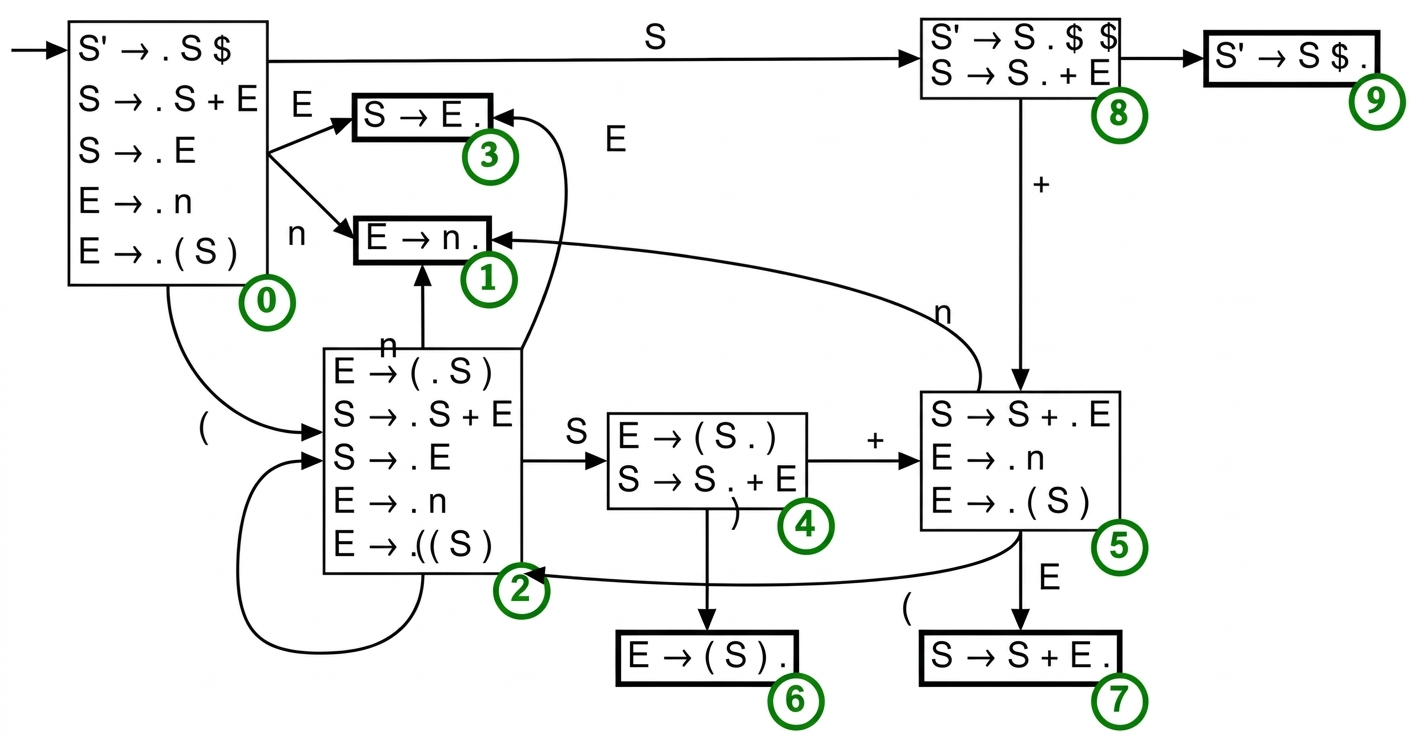
\includegraphics[width=\textwidth,height=0.82\textheight,keepaspectratio]{chapter09/imgs/lr0.png}
\end{frame}

\begin{frame}[fragile]{Regras de Preenchimento LR(0)}
\protect\hypertarget{regras-de-preenchimento-lr0}{}
\begin{itemize}

\item
  \textbf{Shift}: para terminal \(t\) após o ponto em item do estado
  \(i\):

  \begin{itemize}

  \item
    \texttt{action[i, t] = Shift j} onde \(j\) = índice
    de \texttt{goto(i, t)}
  \end{itemize}
\end{itemize}
\end{frame}

\begin{frame}[fragile]{Regras de Preenchimento LR(0)}
\protect\hypertarget{regras-de-preenchimento-lr0-1}{}
\begin{itemize}

\item
  \textbf{Reduce (LR0)}: para item completo \(A \to \alpha .\) no estado
  \(i\):

  \begin{itemize}

  \item
    \texttt{action[i, t] = Reduce(A → α)} para
    \textbf{todos} os terminais \(t\)
  \item
    LR(0) ignora completamente o lookahead nas redu\c{c}\~{o}es!
  \end{itemize}
\end{itemize}
\end{frame}

\begin{frame}[fragile]{Regras de Preenchimento LR(0)}
\protect\hypertarget{regras-de-preenchimento-lr0-2}{}
\begin{itemize}

\item
  \textbf{Accept}: quando o item completo é \(S' \to S .\):

  \begin{itemize}

  \item
    \texttt{action[i, $] = Accept}
  \end{itemize}
\end{itemize}
\end{frame}

\hypertarget{slr-simple-lr}{%
\section{SLR: Simple LR}\label{slr-simple-lr}}

\begin{frame}{O Problema do LR(0)}
\protect\hypertarget{o-problema-do-lr0}{}
LR(0) ignora o lookahead → gera muitos conflitos shift-reduce

\textbf{Exemplo:} gramática com recurs\~{a}o \`{a} direita

\[E \to T + E \mid T \quad T \to n \mid (E)\]
\end{frame}

\begin{frame}[fragile]{O Problema do LR(0)}
\protect\hypertarget{o-problema-do-lr0-1}{}
\begin{itemize}
\item
  Estado com \(E \to T .\) e \(E \to T . + E\):
\item
  Item completo \(E \to T .\) → LR(0) insere reduce em \textbf{todos} os
  terminais, inclusive \texttt{+}
\item
  Item \(E \to T . + E\) → exige shift em \texttt{+}
\item
  \textbf{Conflito!}
\end{itemize}
\end{frame}

\begin{frame}{A Solu\c{c}\~{a}o SLR}
\protect\hypertarget{a-soluuxe7uxe3o-slr}{}
\textbf{Ideia}: reduzir \(A \to \alpha\) faz sentido apenas quando o
próximo token pode seguir \(A\) na gramática

\[\text{reduce apenas em } t \in \mathrm{FOLLOW}(A)\]
\end{frame}

\begin{frame}[fragile]{A Solu\c{c}\~{a}o SLR}
\protect\hypertarget{a-soluuxe7uxe3o-slr-1}{}
Para \(E \to T .\) com \(\mathrm{FOLLOW}(E) = \{\$, )\}\):

\begin{itemize}

\item
  LR(0): insere reduce em todos os terminais (inclusive
  \texttt{+})
\item
  SLR: insere reduce apenas em \texttt{$} e
  \texttt{)} --- sem conflito com shift em
  \texttt{+}!
\end{itemize}
\end{frame}

\begin{frame}{Exemplo SLR}
\protect\hypertarget{exemplo-slr}{}
\[\begin{array}{lcl}
E &\to& E + T \mid T \\
T &\to& T * F \mid F \\
F &\to& (E) \mid n
\end{array}\]
\end{frame}

\begin{frame}[fragile]{Exemplo SLR}
\protect\hypertarget{exemplo-slr-1}{}
Estado com \(E \to T.\) e \(T \to T . * F\):

\begin{itemize}

\item
  LR(0): conflito shift-reduce em \texttt{*} (reduce
  \(E \to T\) e shift de \texttt{*})
\item
  SLR: \(* \notin \mathrm{FOLLOW}(E) = \{+, ), \$\}\)

  \begin{itemize}

  \item
    \texttt{action[estado, *]} recebe apenas Shift ---
    \textbf{sem conflito!}
  \end{itemize}
\end{itemize}
\end{frame}

\hypertarget{conclusuxe3o}{%
\section{Conclus\~{a}o}\label{conclusuxe3o}}

\begin{frame}{Conclus\~{a}o}
\protect\hypertarget{conclusuxe3o-1}{}
\begin{itemize}

\item
  \textbf{Análise bottom-up} é mais expressiva que top-down

  \begin{itemize}

  \item
    Suporta recurs\~{a}o \`{a} esquerda
  \item
    Decis\~{a}o após prefixo maior
  \end{itemize}
\end{itemize}
\end{frame}

\begin{frame}{Conclus\~{a}o}
\protect\hypertarget{conclusuxe3o-2}{}
\begin{itemize}

\item
  \textbf{Earley}: analisa qualquer GLC, \(O(n^3)\) no pior caso
\item
  \textbf{LR(0)}: aut\^{o}mato de estados × itens, tabela de a\c{c}\~{o}es/goto
\item
  \textbf{SLR}: melhora LR(0) restringindo reduces a
  \(\mathrm{FOLLOW}(A)\)
\end{itemize}
\end{frame}
